\section{Three Dimensional Analysis}
\noindent This section extends the analysis of the two dimensional approach, and is intended to explore and analyse the effect of the three dimensional flow features. It was surmised that three dimensional flow allows for more complex flow behaviour, that may significantly affect an undertray's overall performance. This part of the report will be divided into 3D open flow, and analysis of an undertray prototype with bluff body.

\subsection{3D Open Flow}
This analysis is an extension to three dimensions of the 2D open flow cases. The purpose of this analysis to investigate in more detail the flow features that develop in an undertray in a three dimensional manner, which might plausibly affect performance.

\subsubsection{Geometry and Mesh Generation}
An identical 2D sketch from geometry 3 of the 2D open flow section was used, which was then extruded to a car-realistic thickness of 1 meter. A skirt was then added to both sides of the rear diffuser. These skirts are used to improve flow isolation and to generate corner vortices, which help to maintain flow attachment within the diffuser region. Fences were also added to later analyses to investigate the effects of vortex generators with respect to the generation of downforce. A sketch of the geometry can be seen in Figure~\ref{fig:3D_OF_GEOM} below. 

\begin{figure}[!h]
    \centering
    \noindent\makebox[\textwidth]{
    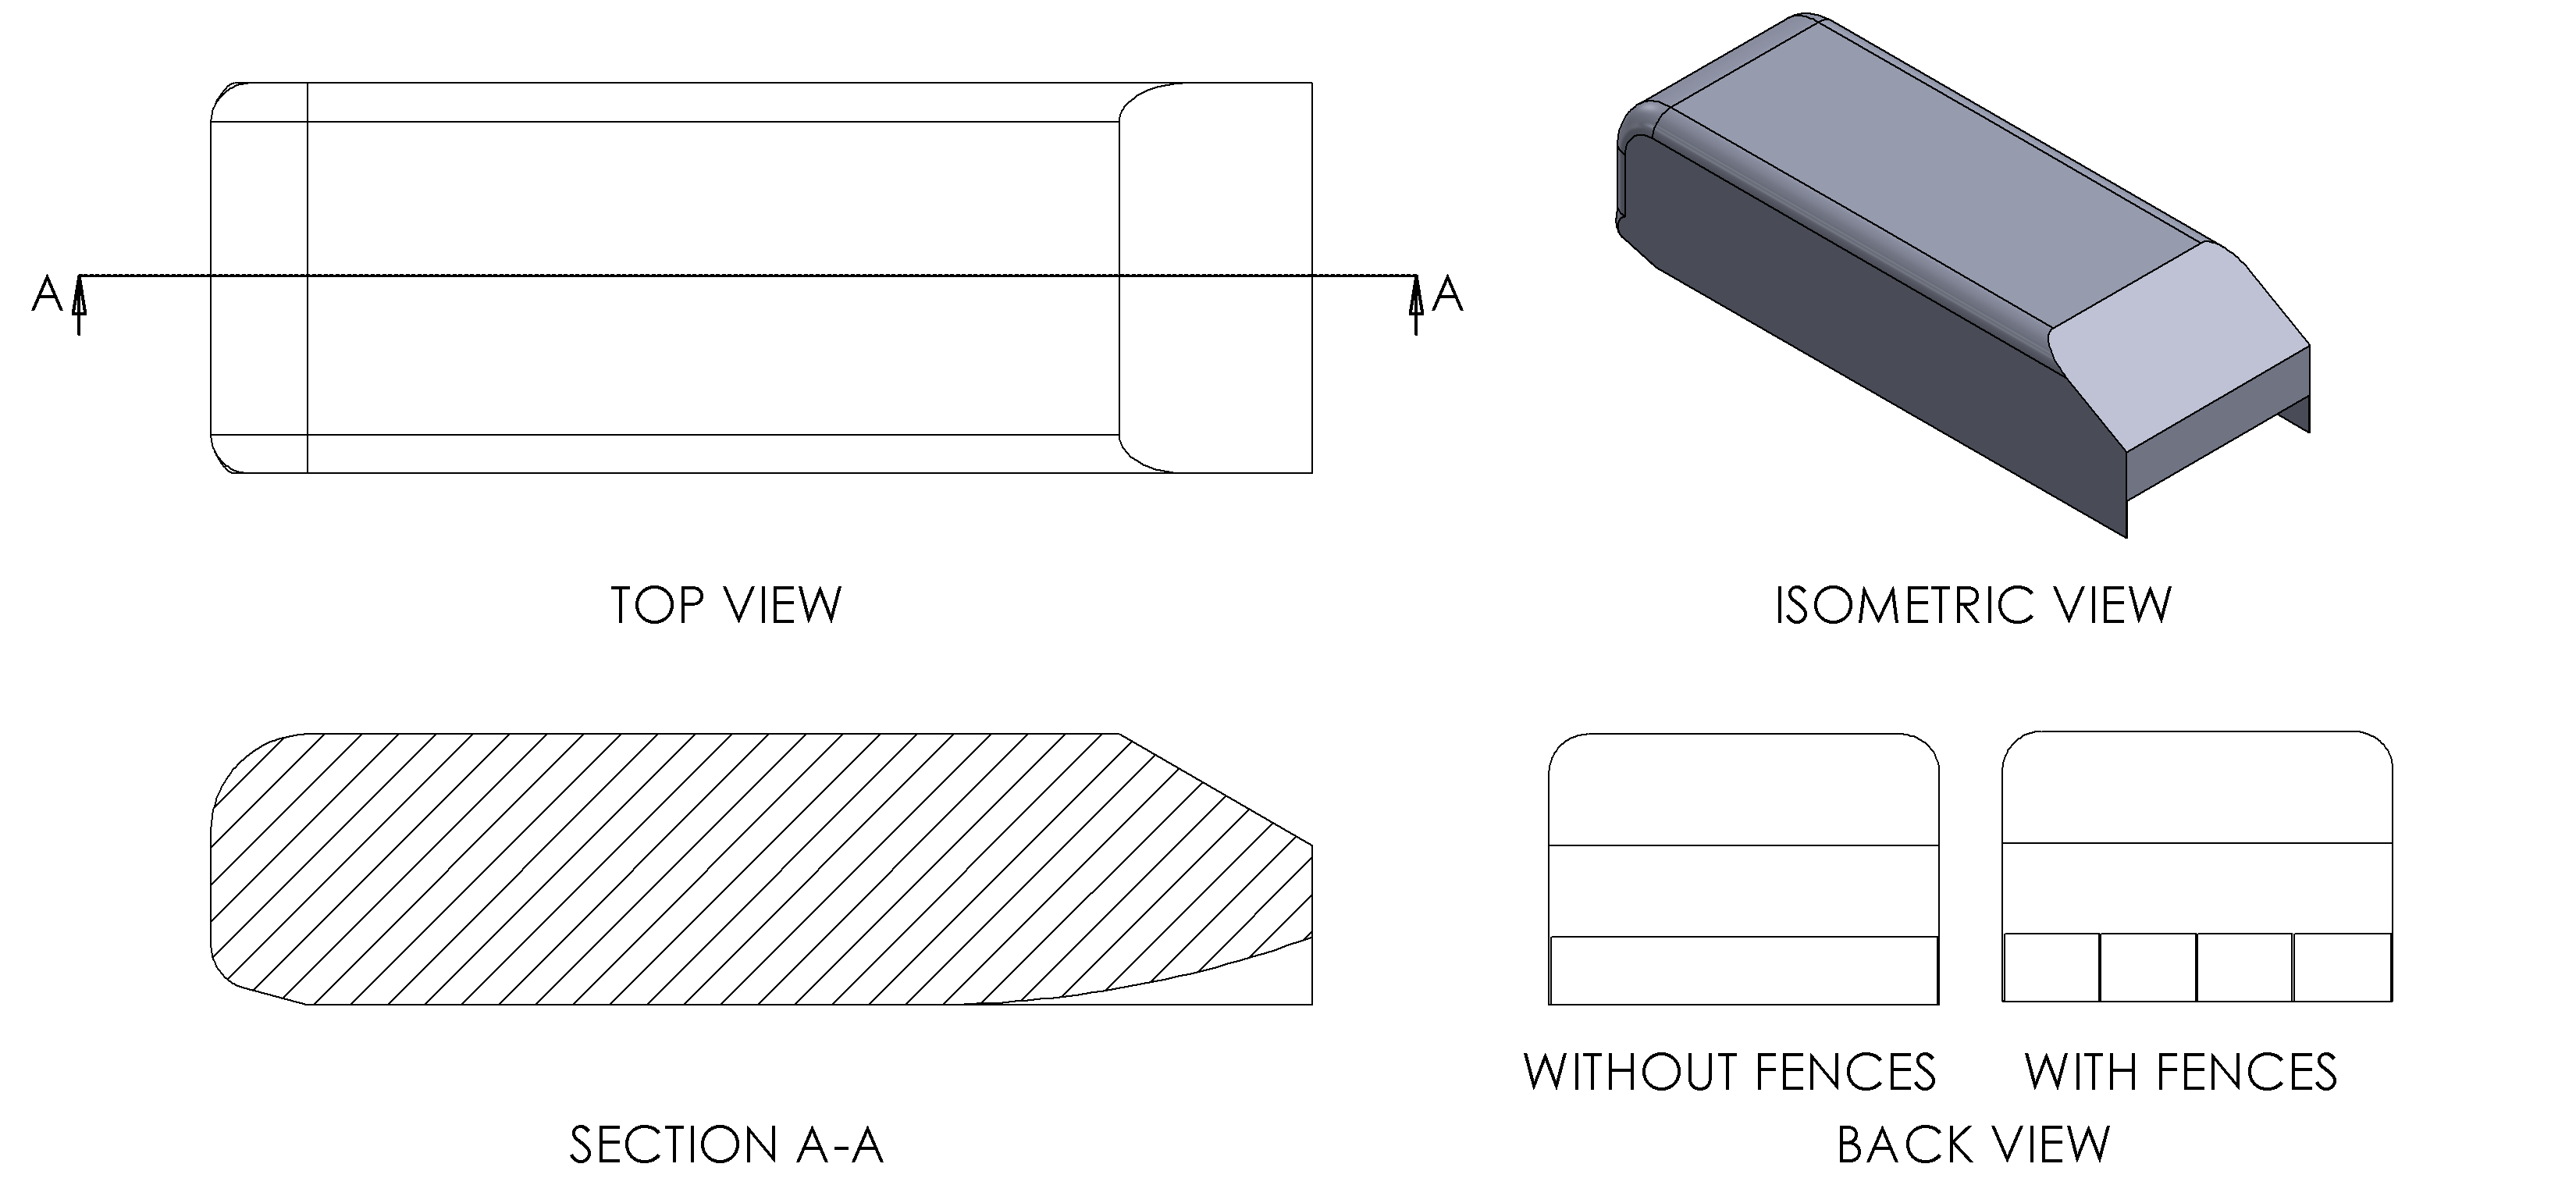
\includegraphics[width=0.8\textwidth]{Figures/3D_OF/3D_OF_D.PNG}}
    \caption{Geometry Generated for 3D Open-Flow Analysis.}
    \label{fig:3D_OF_GEOM}
\end{figure}

\noindent The CAD geometry was then imported into DesignModeler, where the fluid domain and body of influence were built. The fluid domain was made with roughly 2 cars length forward, 5 behind, 3 above, and 3 laterally, with 0.03 meters of ground clearance from the undertray's lowest point. Due to the symmetry of the body, a half model was used for the fluid domain to minimise the mesh element count. A body of influence (BOI), with dimensions of  $6 \times 1 \times 7$ meters was created using a box feature around the body to locally increase the mesh density and capture the surrounding flow features.

\noindent A hybrid mesh was used, which is comprised of tetrahedrons and triangular prisms. Twenty inflation layers of triangular prisms were applied near the wall to give a $y^+=1$. A max element size of 0.8 meters and 0.02 meters in the BOI generated a mesh with 1.3 to 1.5 million elements for this case. The mesh quality is considered acceptable, with an average skewness of 1.9 and an aspect ratio of 80-90; however, a significant jump in size in the cells between the inflation layer and far-field fluid domain is considered not ideal. A detailed illustration of the fluid domain and the mesh can be seen in Figure~\ref{fig:3D_OF_MESH} Appendix C.

\subsubsection{Results and Discussions}
Due to the nature of the mesh, the $k-\omega$ SST model was used throughout this analysis to take advantage of the features of this particular transport model \cite{Ansys2006ModelingFlows}. The analyses will be grouped into four sets of geometries: varying diffuser angle with no inlet angle, varying diffuser angles with an inlet angle of 10 degrees, varying inlet angle with 10 degrees diffuser angle, and variable diffuser angle with three fences applied. Figure~\ref{fig:3D_OF_PLOT_COMPARE_ALL} below shows the comparison of lift and drag between all the variables.

\begin{figure}[htb!]
    \centering
    \noindent\makebox[\textwidth]{
    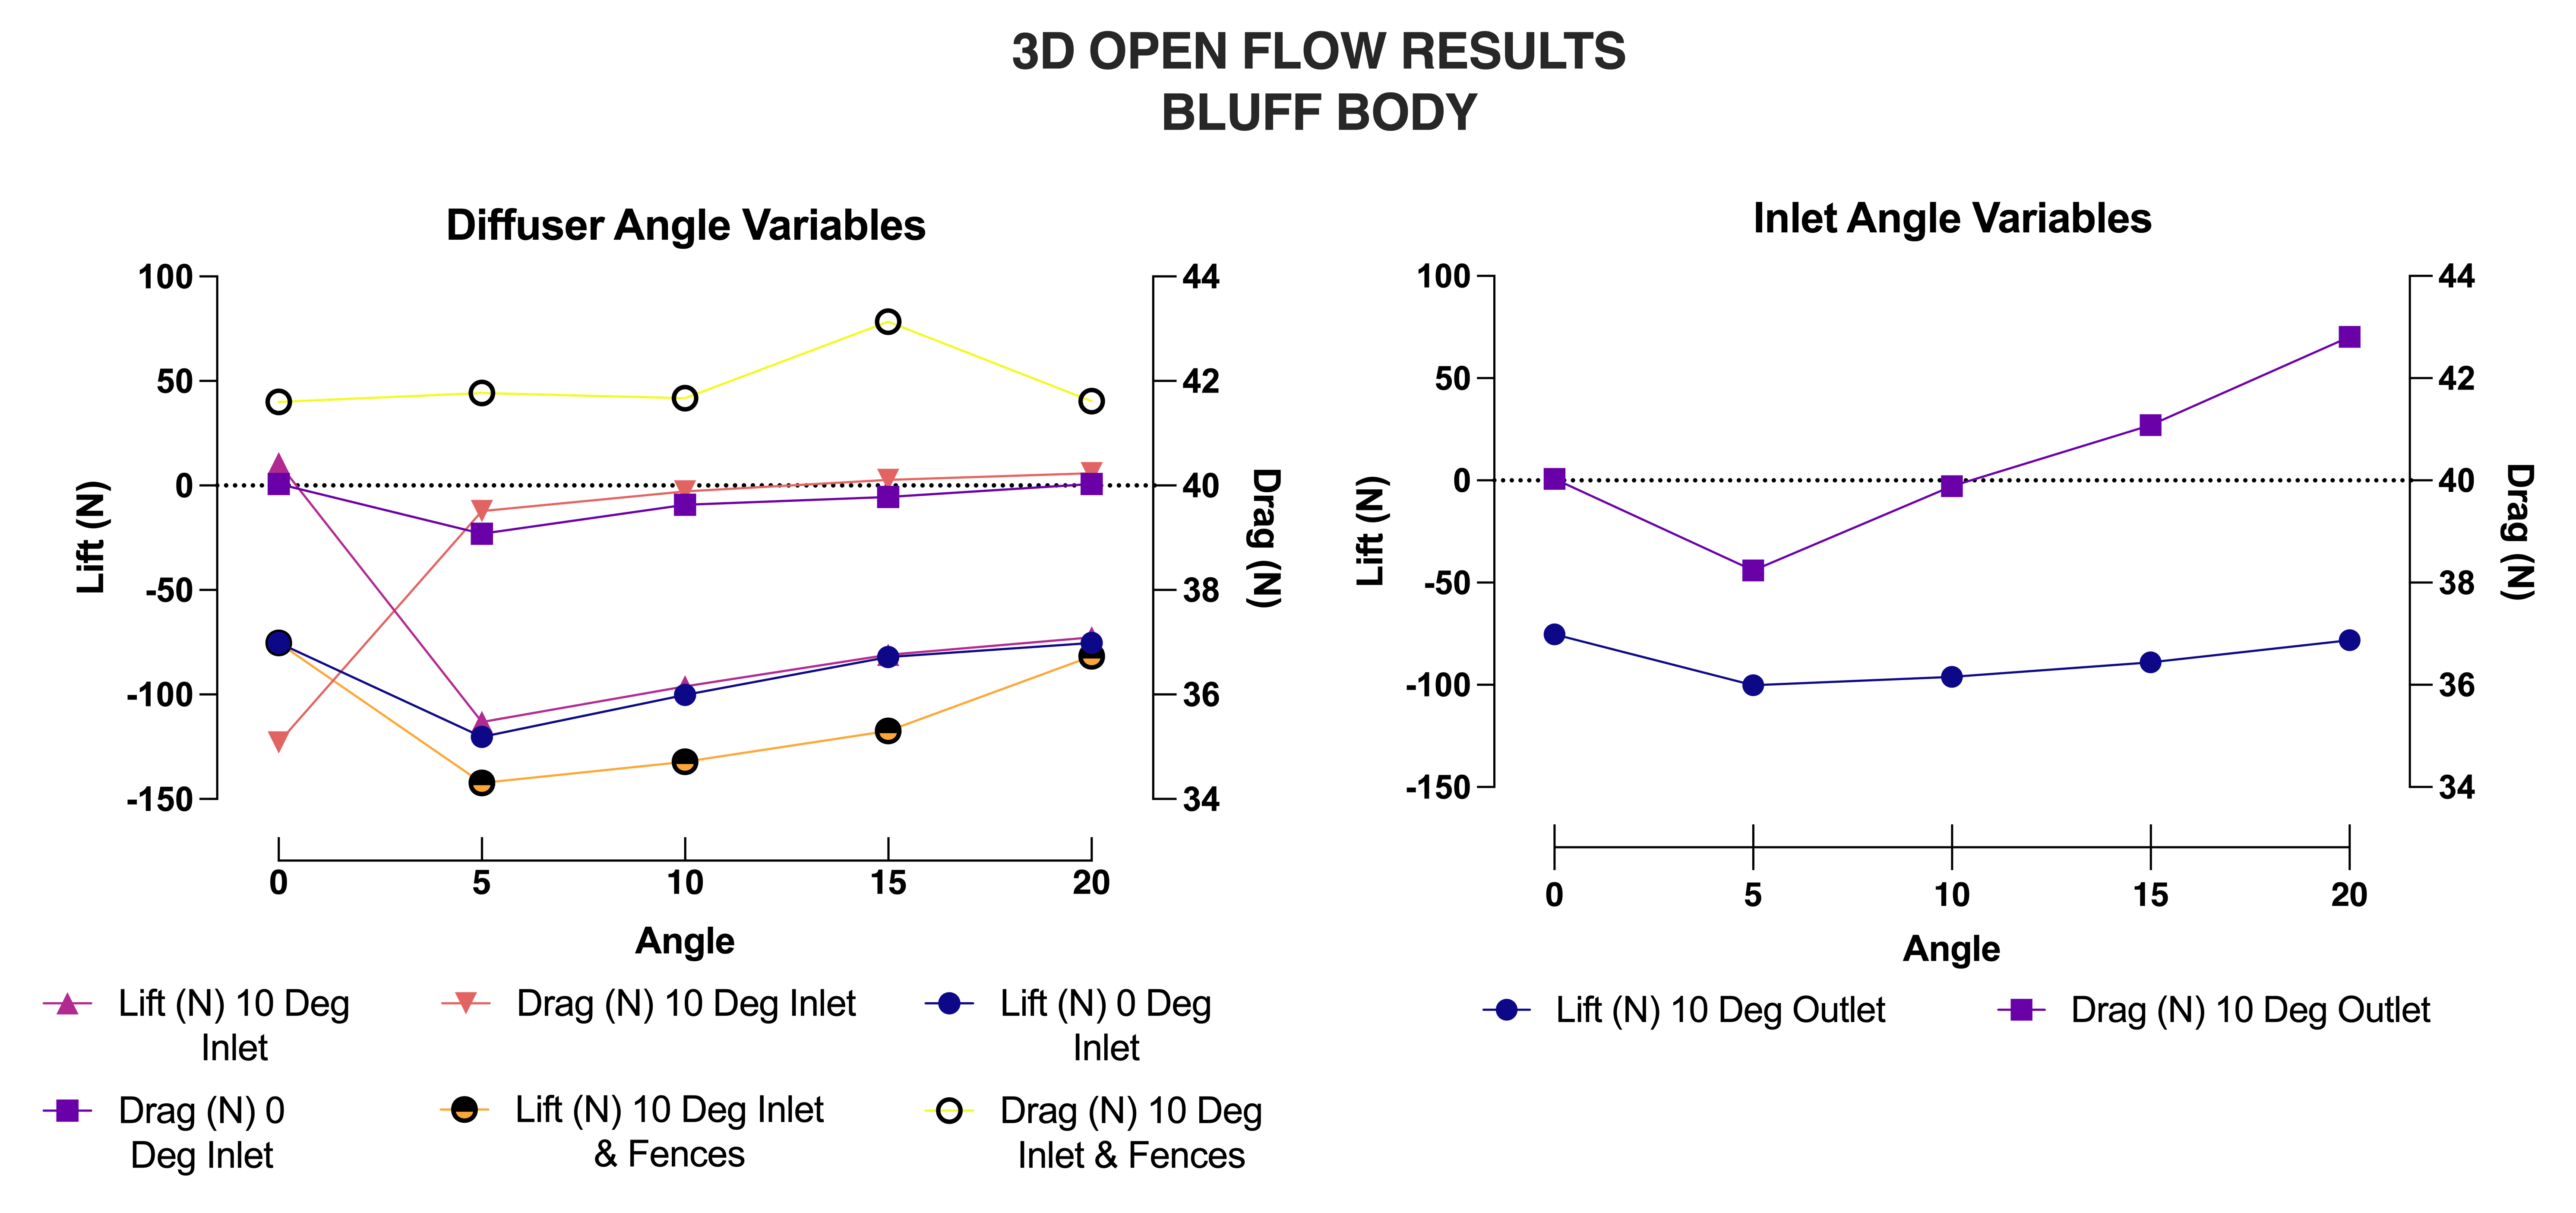
\includegraphics[width=0.95\textwidth]{Figures/Graph/3D_OF.png}}
    \caption{Lift and Drag Variation of Diffuser (left) and Inlet (right) Angle for All Geometry Configurations.}
    \label{fig:3D_OF_PLOT_COMPARE_ALL}
\end{figure}

\noindent The values of lift and drag as computed represent the values for the half body. Once more, a similar trend emerged as with the 2D open flow geometry 3. The trend shows an increase in downforce at a 5 degrees diffuser angle, followed by the downforce falling linearly up to 20 degrees. In comparison with 2D open flow analysis, the average downforce of this analysis is significantly lower. This is due to the nature of the analysis which allows the accelerated flow in the undertray to be affected by the flow surrounding the body. This is in contrast to the 2D open-flow, in which the flow past the undertray is constrained to move solely in-plane. 

\noindent In three dimensions, the lower pressure region in the undertray sucks in the air from the side of the car. The flow which is entrained from the side consequently generates instability and separation on the underbody's accelerated flow \cite{Bouferrouk2014OnVehicles}. This phenomenon may reduce the effectiveness of the flow acceleration underneath, resulting in a lower downforce. This occurrence is illustrated in Figure~\ref{fig:Vector_suction_diagram} below, with the influence of the corner vortices occurring from the fore of the bluff body. 

\begin{figure}[!htb]
    \centering
    \noindent\makebox[\textwidth]{
    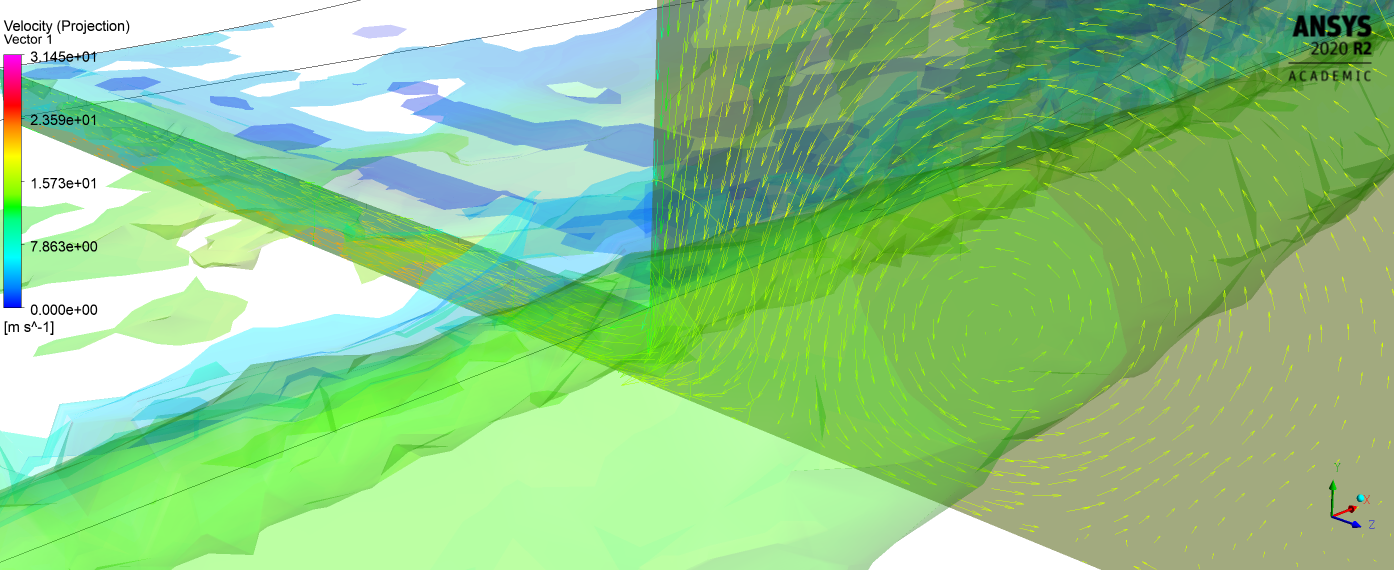
\includegraphics[width=0.8\textwidth]{Figures/3D_OF/3D_OF_VECTOR_SUCTION.png}}
    \caption{Vector Diagram of Velocity Flow on the Undertray's Cross-Section Indicating Flow Suction From The Side of The Body.}
    \label{fig:Vector_suction_diagram}
\end{figure}

\noindent The effect of inlet angle variation was tested with a fixed 10 degree diffuser angle. It can be seen that the effect of changing the inlet angle in 3D shows significant differences to the 2D analyses. The lift and drag of the bluff body reach their minimum at 5 degrees, which is then followed by lift and drag rises up until 20 degrees. As discussed earlier, the stagnation point on the fore of the bluff body in the 2D simulation creates a separation point at which flow is directed to the top and bottom. However, in the 3D case, the stagnation point separates the flow regions less distinctly, which creates more complex flow features around the inlet region. Figure \ref{fig:3D_OF_INLET_COMPARE} left shows the streamline separation from around the surrounding body. Moreover, some of the flow leaks around the side, creating a trailing corner vortex (middle), and hence reducing the intake acceleration in the undertray. In the two dimensional analysis, the flow goes through the undertray without leaking or generating a trailing vortex, improving the flow intake. This explains the downforce degradation after 5 degrees --- as the inlet angle increases, more airflow leaks in the inlet region and creates a bigger trailing vortex. The increase in drag comes from the skin friction as the flow acts over a larger area with elevation of angle, and the trailing vortex can plausibly affect the flow on the throat (as discussed previously). It is worth noting that the change of drag with inlet angle elevation is fairly insignificant and can be ignored.

\begin{figure}[!htb]
    \centering
    \noindent\makebox[\textwidth]{
    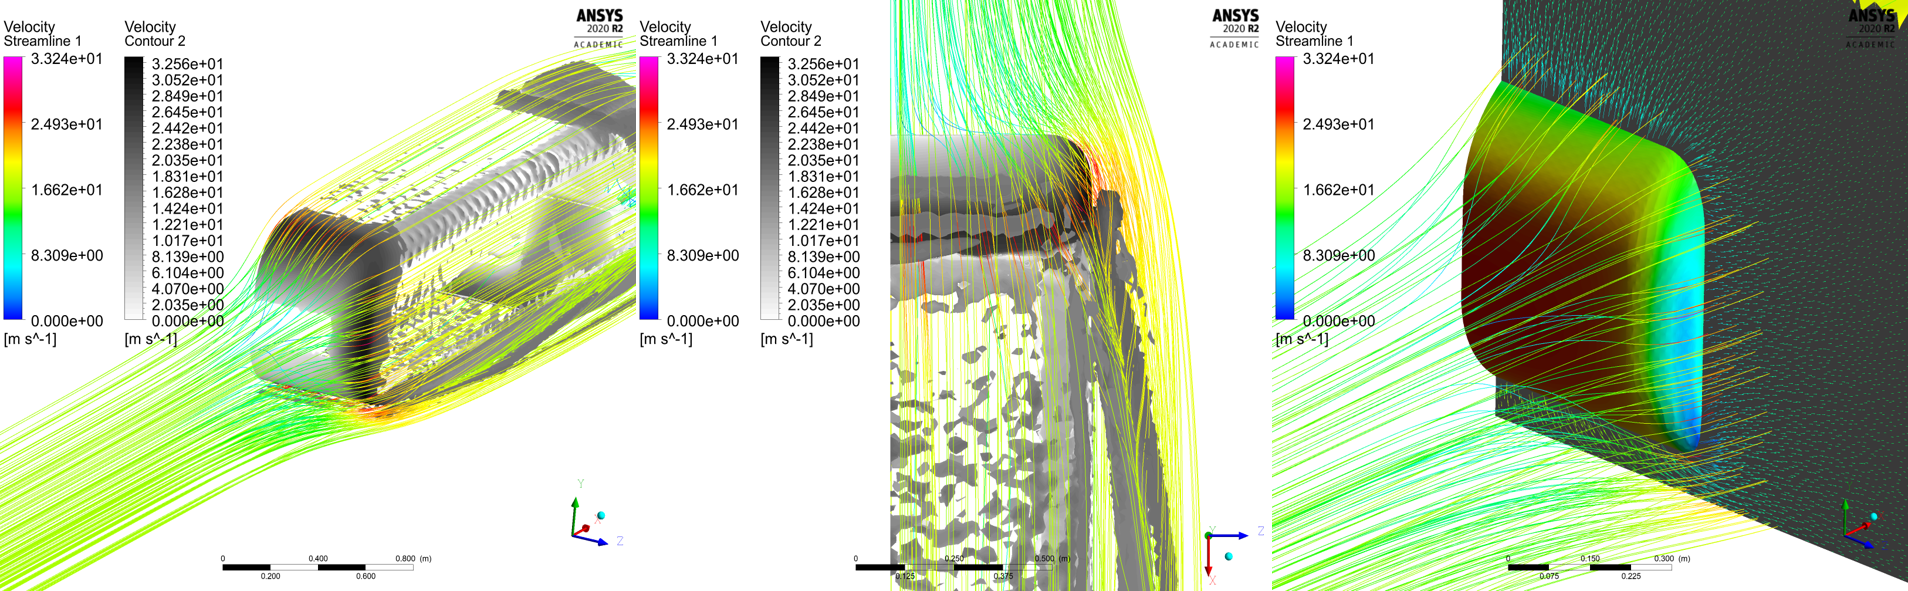
\includegraphics[width=1\textwidth]{Figures/3D_OF/3D_OF_INLET_COMPARE.png}}
    \caption{Fore-Flow Streamline Imposing The Bluff-Body and Occurrence of Leaking Indicated by The Trailing Vortex ($Q$-Criterion Isosurface) at The Inlet Region (left and middle), and Velocity Vector of The Flow Indicating Flow Leaks at The Inlet Region (right).} 
    \label{fig:3D_OF_INLET_COMPARE}
\end{figure}

\noindent Comparing the lift and drag with the diffuser varying with or without an inlet angle, the graphs exhibit identical results except at 0 degrees. Here, there is a noticeable drop in downforce and drag, which is plausibly due to the diffuser's absence. A well-designed diffuser is important because it slowly expands the flow and allows the jet to stay attached to the undertray surface. Moreover, the side skirts in the diffuser allow the generation of corner vortices that help the flow to remain attached still further, hence increasing the overall downforce. ANSYS Post CFD allows the visualisation of $Q$-Criterion isosurfaces, which mark a vortex region ($Q > 0$) as areas of flow where the anti-symmetric component of the velocity gradient tensor dominates the symmetric \cite{Holmen2012MethodsIdentification}. The corner vortex allows the boundary layer to stick on to the wall, slowing the expansion, hence the reduction in lift and drag. This phenomenon can be seen in Figure~\ref{fig:3D_OF_COMPARE_FENCES_SHEAR}, where the region in which the vortex is present has a higher wall shear stress than its surroundings, indicating flow attachment in the respective direction.

\begin{figure}[!htb]
    \centering
    \noindent\makebox[\textwidth]{
    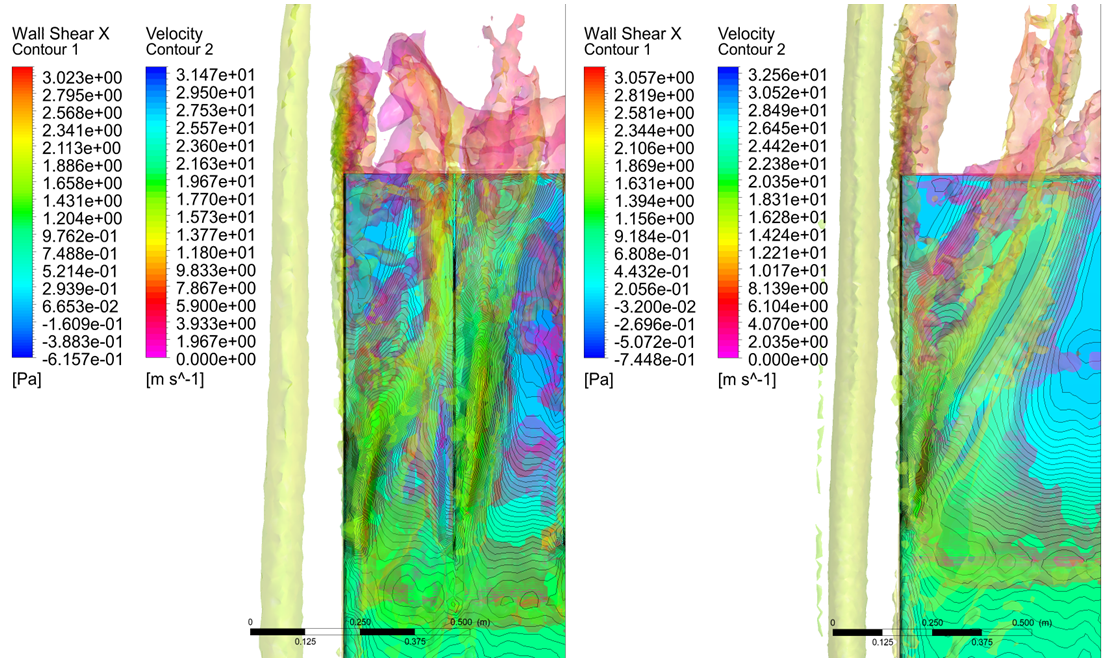
\includegraphics[width=0.65\textwidth]{Figures/3D_OF/3D_OF_COMPARE_FENCES.png}}
    \caption{Comparison of $x$ Wall-Shear and Vortex Velocity ($Q$-Criterion Isosurface) Generated on The Diffuser Region With (left) and Without (right) Fences Applied.}
      \label{fig:3D_OF_COMPARE_FENCES_SHEAR}
\end{figure}

\noindent The next analysis incorporates fences (vertical partitions on the diffuser) to generate corner vortices to investigate their effects on the undertray's performance. The lift and drag plots shown in Figure~\ref{fig:3D_OF_PLOT_COMPARE_ALL} demonstrate an overall higher downforce compared to the bluff body without the fences. A similar concept of vortex generation applies. With the fences installed, there are more vortices generated along the diffuser. This reduces the flow separation in the $x$ direction (the flow direction), and maintains flow attachment, thus increasing the downforce. Figure~\ref{fig:3D_OF_COMPARE_FENCES_SHEAR} illustrates the presence of the extra vortices generated inside the diffuser by additional fences, and the smaller flow separation region indicated by non zero x-wall shear region. 

\subsection{3D Undertray}
Overall, the previous analyses have given a fundamental understanding of the flow behaviour, features, and performance trends of an underbody flow. This section of the report will utilise previous simulations to design several undertray prototypes that will be simulated using a traced bluff-body of the QFR car to achieve a realistic picture of the flow in real-life circumstances. The results are documented and then analysed thoroughly.

\subsubsection{Geometry and Mesh Generation}
\noindent Previous results have developed knowledge of the trends in flow behaviour for the undertray's inlet and diffuser angles. Eight prototype designs have been made based on interpreting these results, along with some engineering judgement from prior results. Several configurations were used to achieve the best results in the designs, including side diffuser, flat side-plate; dual variable diffuser; Gurney flaps; and variable vortex generators. These variables were all aimed at achieving the maximum performance of the undertray. All eight undertray prototype geometries can be seen in Figure~\ref{fig:UTP_D} in Appendix D.

\noindent An earlier project by McClune \cite{McClune2018DesignCar} analysed several undertray designs. However, the simulations undertaken consisted solely of the undertray; hence, unrealistic velocity and pressure fields were developed on the top surface of the undertray. To overcome this issue, A bluff-body traced from the actual car was developed and installed to approximate the real QFR 2021 car. Nonetheless, several simplifications were made for ease and computational performance, such as removing the suspension and tyres, which may disturb or pre-sculpt the oncoming flow before it enters the side undertray. Figure~\ref{fig:3D_UT_BB_SIMPLIFICATION} shows the QFR car simplification into a bluff body that fits above the undertray design.

\begin{figure}[!htb] 
    \centering
    \noindent\makebox[\textwidth]{
    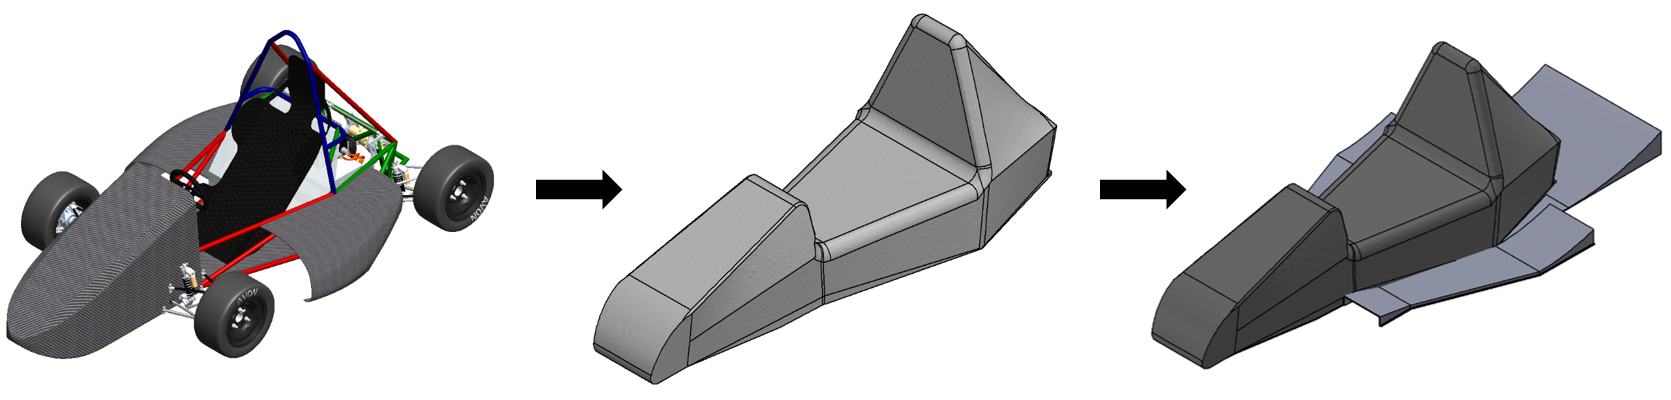
\includegraphics[width=0.8\textwidth]{Figures/UTP_FIGS/UT_BB_SIMPLIFY.png}}
    \caption{Simplification of QFR Car as an Undertray's Bluff Body to Simulate Realistic Flow Around The Body.}
      \label{fig:3D_UT_BB_SIMPLIFICATION}
\end{figure}

 \noindent A computational domain was then generated using Design Modeller. A fluid-flow region enclosing one symmetrical half of the car was made, with the domain extending roughly 3 cars length behind, 1 forward, 1 on top, and 1 to the side, with a 0.03 meters clearance gap from the lowest point of the undertray. To refine the mesh and help capture the flow features in the undertray and bluff-body regions, two Bodies of Influence (BOIs) were incorporated. A bigger BOI, with dimensions of 5 $\times$ 1.2 $\times$ 1.2 meters was generated to capture the flow surrounding the bluff body, and an additional smaller BOI on the undertray region was 3 $\times$ 0.25 $\times$ 0.7 meters. The enclosed fluid flow generated can be seen in Figure \ref{fig:UTP_Fluid_flow} in Appendix D
 
 \begin{figure}[!htb] 
    \centering
    \noindent\makebox[\textwidth]{
    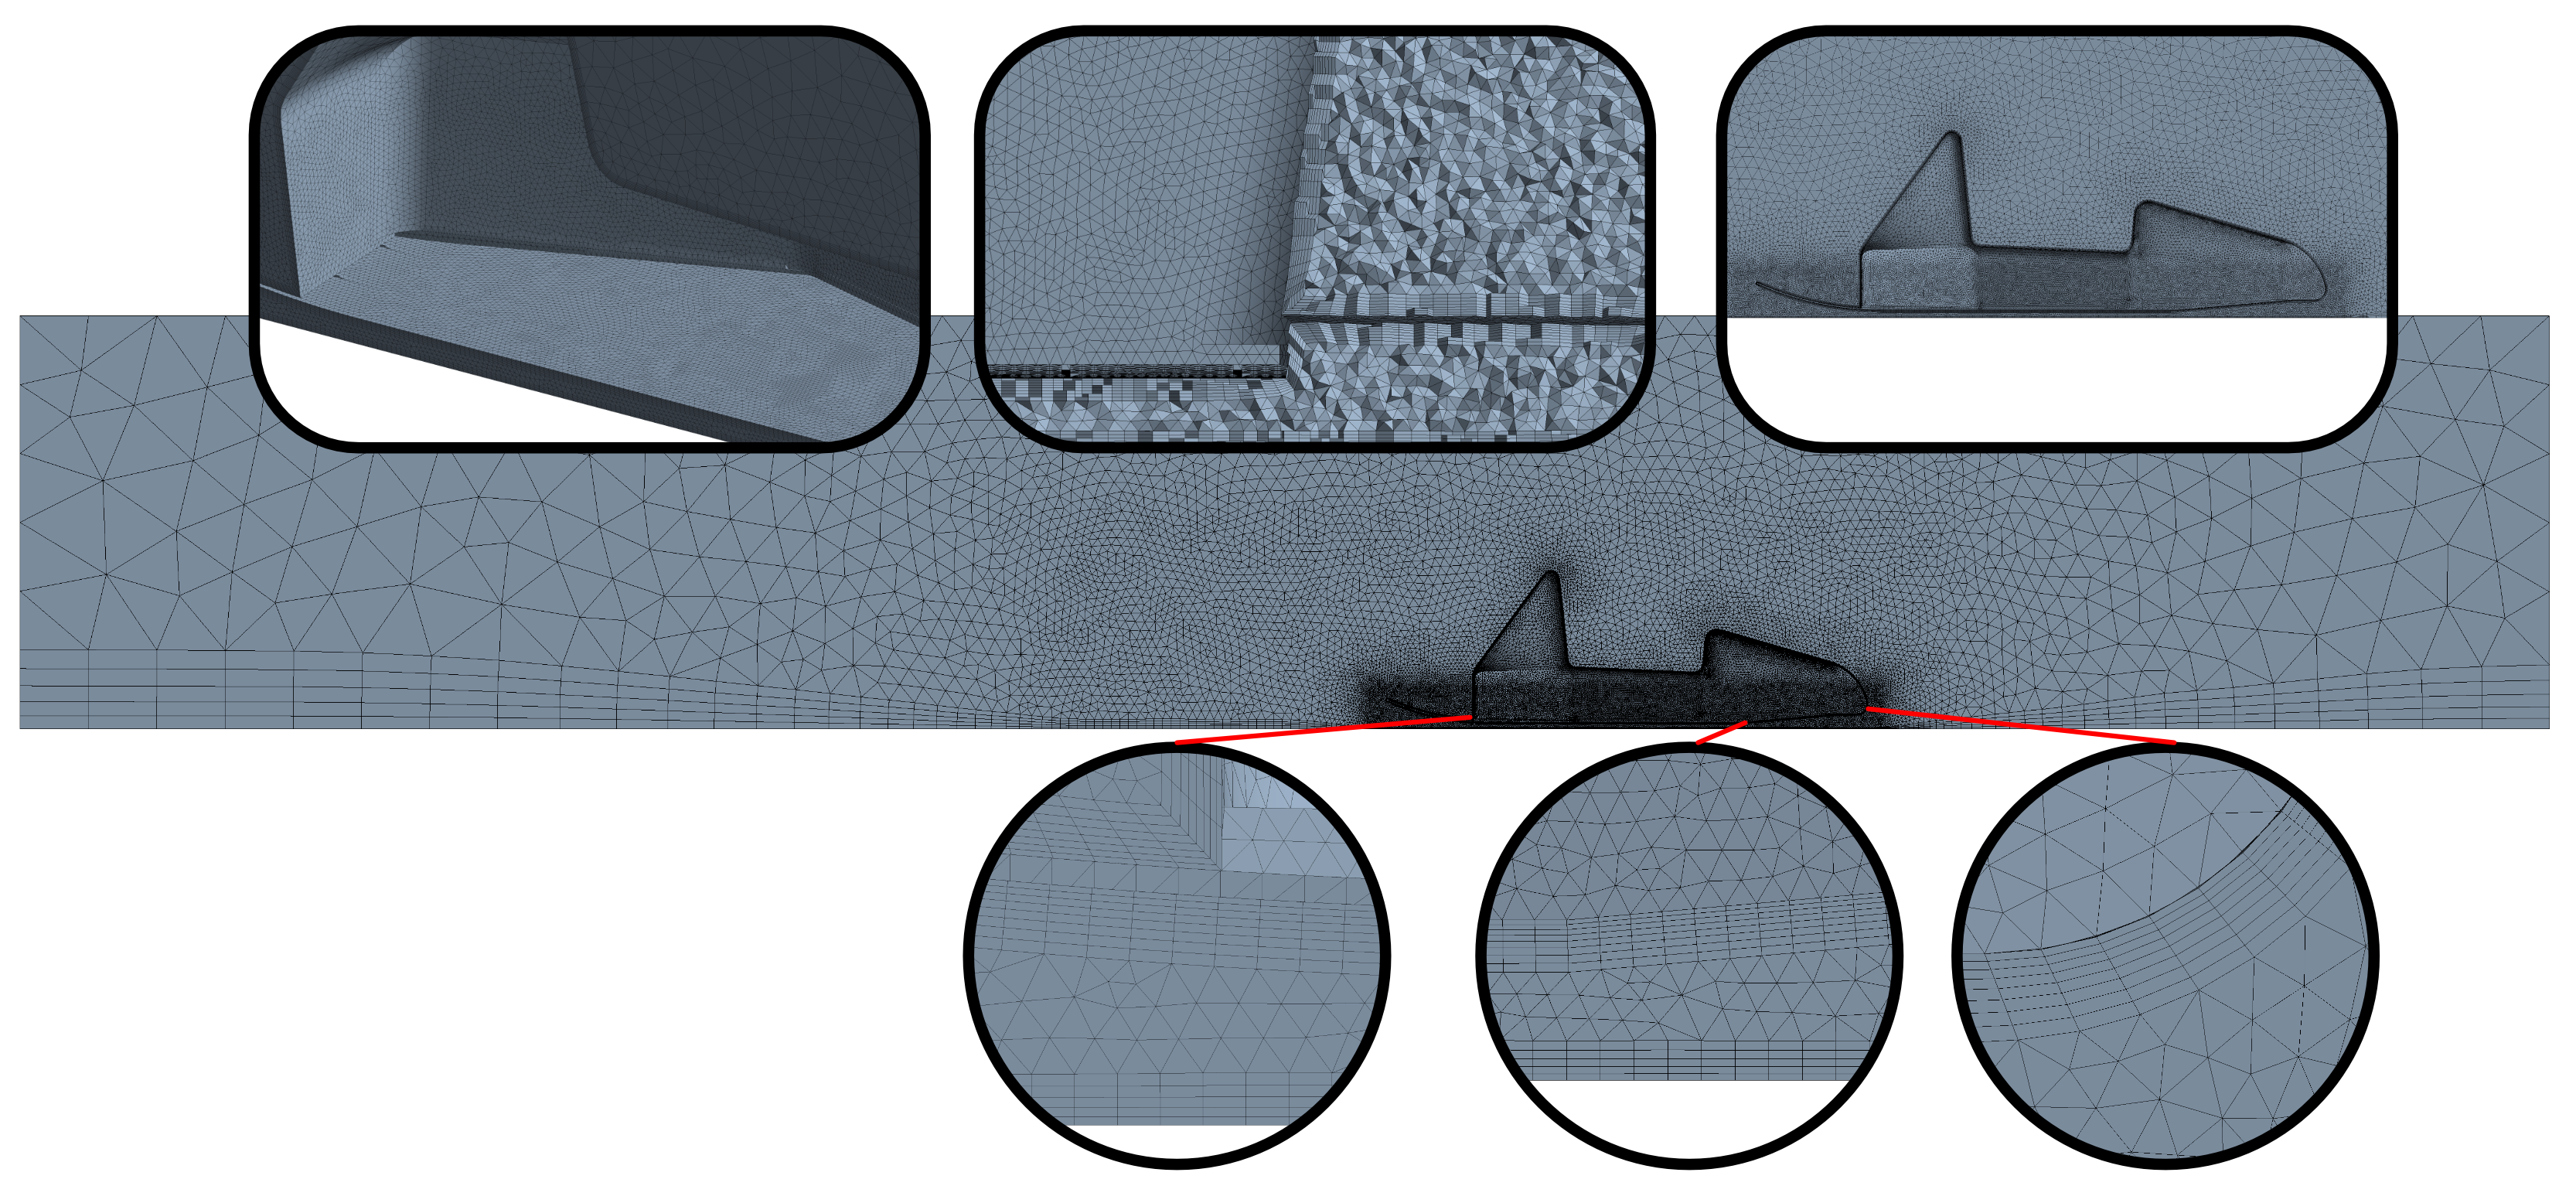
\includegraphics[width=0.9\textwidth]{Figures/UTP_FIGS/3D_UT_BB_MESH_COMPILE.png}}
    \caption{3D Hybrid Mesh Generated for Undertray Prototype Design With Bluff Body.}
    \label{fig:3D_UT_MESH}
\end{figure}

\noindent A hybrid mesh for the 3D Undertray Prototype design is shown in Figure~\ref{fig:3D_UT_MESH}. To capture details on the undertray region, 2 BOIs were used on both car's surroundings and on the undertray area. The first BOI used minimum element sizing of 0.05 meters of sizing, and the second used 0.008m near the undertray region, with a cell growth rate of 1.1. In a similar manner to the other analyses, inflation layers were used on the moving floor and bluff body surfaces. $y^+ = 1$ was used near the body, with 8 inflation layers, a first cell height of 0.00115 meters, and a cell growth rate of 1.1. However, to reduce the jump in cell size after the inflation region to the far-field and still capture the boundary layer in the undertray region, a smooth transition inflation layer was used in the floor region. A smooth transition of 0.272 (the default value) with five inflation layers and the same cell growth rate of 1.1 was used. This resulted in meshes of around 9.5 to 9.8 millions elements being generated, with an average element quality of 0.785, a skewness of 0.206, and an aspect ratio of 2.399, which put the overall quality of the mesh in a very good region \cite{Ansys2006ModelingFlows}.   

\subsubsection{Results and Discussion}
Table \ref{UTB_RESULTS} below shows the eight undertray simulation results for comparison, calculated with similar simulation environments and settings. The bluff body alone was also simulated to act as the baseline for comparison against cases with designed undertrays attached. Note that UTP stands for Undertray Prototype in the simulation and file naming convention.


\begin{table}[!htb]
\centering
\caption{Simulation Results of Undertray Prototype Designs.}\label{UTB_RESULTS}
\begin{tabularx}{0.95\textwidth}{ 
  | >{\centering\arraybackslash}X 
  | >{\centering\arraybackslash}X
  | >{\centering\arraybackslash}X
  | >{\centering\arraybackslash}X
  | >{\centering\arraybackslash}X
  | >{\centering\arraybackslash}X |
  }
\hline
\multirow{2}{*}{Design Name} & \multicolumn{2}{>{\hsize=\dimexpr2\hsize+2\tabcolsep+\arrayrulewidth\relax\centering}X|}{Full Body Results}  & \multirow{2}{*}{L/D Ratio} & \multicolumn{2}{>{\hsize=\dimexpr2\hsize+2\tabcolsep+\arrayrulewidth\relax\centering}X|}{Aerodynamics Improvement} \\ \cline{2-3} \cline{5-6}
 & Lift (N) & Drag (N) & & Lift (N) & Drag (N) \\
\hline

Bluff Body (Baseline)& -38.48 & 78.72 & -0.49 & 0 & 0\\
\hline
UTP0 & -106.26 & 59.81 & -1.78 & -67.79 & -18.91\\
\hline
UTP1 & -124.00 & 80.78 & -1.53 & -85.50 & 2.06\\
\hline
UTP2 & -222.59 & 68.23 & -3.26 & -184.12 & -10.49\\
\hline
UTP3 & -108.40 & 67.15 & -1.61 & -69.92 & -11.57\\
\hline
UTP4 & -136.75 & 72.60 & -1.88 & -98.28 & -6.12\\
\hline
UTP5 & -225.83 & 80.50 & -2.81 & -187.36 & 1.78\\
\hline
UTP6 & -224.23 & 81.00 & -2.77 & -185.76 & 2.28\\
\hline
UTP7 & -226.52 & 79.77 & -2.84 & -188.05 & 1.05\\
\hline \hline
UTP2 at 20 km/h & -26.06 & 7.77 & -3.35 & N/A & N/A\\
\hline
UTP2 at 100 km/h & -711.31 & 197.74 & -3.60 & N/A & N/A\\
\hline
\end{tabularx}
\end{table}

\noindent The bluff body acts as a baseline case, which is used to indicate the performance improvement when an undertray is attached. To get an overall performance indicator, the efficiency can be deduced from the lift-to-drag ratio. The design process of the undertrays was incremental; however, some experimental designs were utilised. Several patterns can be seen based on common undertray design features. Firstly, it can be seen that all diffusers have improved the car's performance compared to that of the plain bluff body. Comparing UTP 0, 3, 4 to other geometries shows that including the side-diffuser increases the overall downforce, but not necessarily the aerodynamic efficiency. For instance, UTP1 has higher downforce than either UTP0 or UTP4; however, UTP 1 has the least advantageous value of aerodynamic efficiency. The results have also shown that undertrays with variable diffusers (e.g. UTP4, UTP5, UTP6) have a higher downforce but that this is also directly proportional to their drag. Additional features, such as dual-variable diffuser angles and gurney flaps, as in UTP3-UTP7, do increase the performance slightly; however, it was decided that the the increase in manufacturing complexity made these features unsuitable for inclusion. It is worth mentioning that a curved side-diffuser (a side diffuser that follows the body's curve) is the most prominent extra feature that significantly improves the aerodynamic efficiency. It is observed that UTP2, UTP5, UTP6, and UTP7 values have almost doubled in their efficiency due to the presence of a curved side diffuser.

\noindent Based on the L/D ratio, it was decided that undertray prototype 2 (UTP2) will be used as the QFR car's undertray. It is also shown that UTP2 increases the downforce by 184.12 N (a 678.5\% downforce improvement) and reduces the drag by 10.49 N (a 13\% drag reduction). UTP2 has 0.61 meters of 12 degrees for the diffuser (including six linearly spaced vortex generating fences) and a 1.1 meter side-diffuser, with 10 degree inlet and outlet angles. A technical drawing of the final undertray design (UTP2) can be seen in Figure \ref{fig:UTP2_FINAL_DESIGN} in Appendix D. Other designs such as UTP5-7  have a slightly higher downforce; however, they also generate high values of drag, making their lift to drag ratios lower than UTP2. The lower lift to drag ratio is vital for balancing the undertray performance in both high and low-speed racing.

\begin{figure}[!htb] 
    \centering
    \noindent\makebox[\textwidth]{
    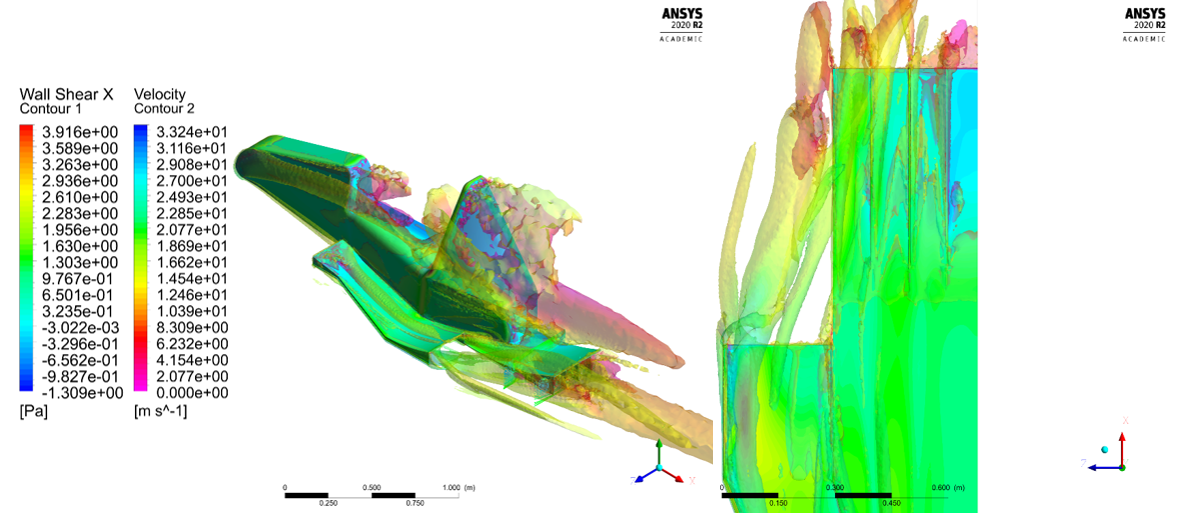
\includegraphics[width=1\textwidth]{Figures/UTP_FIGS/UTP_QCRIT_WSHEAR_COMPILE.png}}
    \caption{Undertray Prototype 2 with Bluff Body $x$ Wall Shear and Velocity Contour of Q-Criterion of 0.005 .}
      \label{fig:3D_QCRIT_WSHEAR_UTP2}
\end{figure}

\noindent Figure~\ref{fig:3D_QCRIT_WSHEAR_UTP2} shows the $x$ wall shear on the bluff body as well as the vortex pattern, as indicated by the Q-Criterion. Similarly to the previous analysis, regions of negative $x$ wall shear indicate the separation region on the undertray. As has been shown previously, flow attachment is a crucial factor in improving the overall performance. Vortices formed at the rear, generated by the vortex generating fences, play a crucial role in determining the undertray's performance. A good undertray design is graded by its effectiveness at capturing or trapping the vortices, which creates a suction effect \cite{Bouferrouk2014OnVehicles}; hence, higher downforce and thus traction can be achieved. It can be seen from Figure~\ref{fig:3D_QCRIT_WSHEAR_UTP2} above that the flow stays attached in the diffuser region where the vortex formed, and the blue region in the middle of the diffuser indicates flow separation taking place where the vortex is not prominent. UTP 2,5,6, and 7 have similar side-diffuser geometries; however, each undertray's diffuser geometry is distinct. UTP 5, 6, and 7 have a higher angle on the outermost section; this allows a larger vortex to be generated, which produced a slight increase in downforce (see Table~\ref{UTB_RESULTS}).

\noindent Nonetheless, ineffective vortex generation, which causes shedding, induced early flow separation of the diffuser's boundary layer, causing a significant drag increase. It can be seen from Figure~\ref{fig:UTP_BOTTOM_QCRIT_ALL_COMPARE} in Appendix D that the outermost region of UTP 5, 6, and 7 shows lower $x$ wall shear values (indicated by the light blue regions), suggesting that flow separation occurred in that region, which generated unstable and shedding vortices, hence resulting in a drag increase. Comparing the undertrays with similar lift values (e.g. UTP 2, 5, 6, and 7), it was suspected from Figures~\ref{fig:UTP_BOTTOM_QCRIT_ALL_COMPARE} and \ref{fig:UTP_ISO_QCRIT_ALL_COMPARE} that the undertrays with higher drag (UTP 5, 6, and 7) had vortices near the outlet that may indicate vortex instability, compared to UTP2 which has a cleaner trailing vortex. Moreover, the curved side diffuser sculpts the inlet's flow laterally, which increases the acceleration and decreases the pressure. This condition generated a sizeable corner vortex and low pressure region at the turning point, increased the trapped vortex's size, and therefore increased the overall downforce.

\noindent However, the simulation used a clean bluff-body which allows clean air to enter the inlet region on both nose and side diffuser. This is not a perfect representation of the real-life case, as several parts, such as the suspension, tyres, and front wing (in future designs), might disturb the incoming flow and ultimately affect the vortex generation at the rear. It can be concluded that downforce improvement and drag reduction is complex a matter of flow management so that effective flow control can achieve a stable vortex using intelligent analysis and advanced undertray designs. Therefore, focusing on stable vortex generation should be the priority for future work in undertray design. Another limitation of the design here is that all the simulations were done in a partial half-model. A paper by Senior \cite{Senior2001TheEffect} illustrated the importance of symmetric flows in high-performance undertrays, and the analyses in this project have naturally enforced a symmetrical flow in the simulation. Hence, in future projects, it is also important that the undertray simulations are done using the whole car geometry.
















